\setcounter{chapter}{12-1} %Makes the prereq chapter chapter 0

\chapter{Markov Decision Processes 2 - Optimal Policies, Q-Values}

\setcounter{section}{1}


\section{Finding policies for MDPs}

    In the previous section, we computed the total value of different \purp{policies}: strategies for how to act, to get the \textbf{most rewards.}

    \begin{itemize}
        \item We designed \vocab{value functions} in order to \gren{evaluate} policies, and find the best one.
        \item So, we'll do that: we search for the \orgg{optimal} policies, in the \textbf{finite} and \textbf{infinite} cases.\\
    \end{itemize}

    \begin{definition}
        The \vocab{optimal policy} \pur{$\pi^*$} is better than (or as good as) every other policy \grn{$\pi$}, for \redd{every state}.

        \begin{equation*}
            \red{\forall s \in \mathcal{S}}: \qquad \qquad 
            V_{\grn{\pi}}(\red{s}) \leq V_{\pur{\pi^*}}(\red{s})
        \end{equation*}

        There can be \gren{multiple} optimal policies.
    \end{definition}

    

    \phantom{}

    \subsection{Optimal Policies -- Finite Horizon, $H=0,1$}

        We could try every possible policy, and compare their \gren{values} directly.

        \begin{itemize}
            \item But that's way too expensive: the number of policies is typically \purp{huge}. 
        \end{itemize}

        Instead, let's do what we did before: we start with the optimal policy for $h=0$, and build up a larger \vocab{horizon}.\\

        \begin{notation}
            Note that our \purp{policy} can depend on our \gren{horizon}. We'll add notation to accommodate this:

            \begin{itemize}
                \item The \vocab{optimal policy} for horizon $h$ is $\grn{\pi}_h^*$.
            \end{itemize}

            
        \end{notation}

        \miniex If it takes 10 steps to reach a very valuable state, you should have a different policy if 

        \begin{itemize}
            \item You have $h=3$ (not enough time to reach it)
            \item You have $h=100$ (more than enough time to reach it)
        \end{itemize}

        \subsecdiv

        First: $H=0$. There's no reward, no matter what we do: all policies are the same.\\

        \begin{concept}
            \purp{All policies} for $h=0$ are \vocab{optimal}.
        \end{concept}

        \subsecdiv

        Next, $H=1$: we only have to take one action. Thankfully, this is simple: we just take the \brow{action} that \purp{maximizes} our reward.

        \begin{itemize}
            \item This looks like a job for \vocab{argmax}.
                \note{In the regression chapter, we discussed argmin, but the principle is exactly the same.}\\
        \end{itemize}

        \begin{notation}
            \textit{Review from the Regression chapter:}
            
            The \vocab{argmax function} tells you the value of the \{input \brow{variable} that gives the \purp{maximum output}.
            
            \begin{equation*}
                \Theta^* = \argmax{ \pur{ \Theta } }{ \grn{ J(\Theta) } }
            \end{equation*}
            
            The \purp{function we want to maximize} is written to the right, while the \brow{variable we adjust} is written below.
        
        \end{notation}

        So, we want to know which \brow{action} maximizes the \purp{reward} function.

        \begin{itemize}
            \item We just compute this by comparing all the actions for a single \redd{state}.
        \end{itemize}

        \begin{equation}
            a^* = \argmax{\bro{a}}{ \Big( R\big( \red{s},\bro{a}\big) \Big) }
        \end{equation}

        If we're in state $\red{s}$, we want our \purp{optimal policy} to give this action.\\

        \begin{kequation}
            The \vocab{optimal policy} for horizon $H=1$ is:

            \begin{equation*}
                \pi^{*}_{1}\big(\red{s}\big) = \argmax{\bro{a}}{ \Big( R\big( \red{s},\bro{a}\big) \Big) }
            \end{equation*}
        \end{kequation}

            \note{Remember that we can have multiple optimal policies.}



    \phantom{}

    \subsection{Finite Horizon: $h=2$}

        Now, we want to find the policy if $H=2$.

        This has a few complications:

        \begin{itemize}
            \item We have to choose \purp{two} separate actions.
            
            \item Our \brow{$h=2$ action} will affect our state (and reward) at $h=1$.
                \begin{itemize}
                    \item So, we can't just choose the \textbf{action} that gives us the best \gren{immediate reward}: we need to account for \textit{future} reward.
                \end{itemize}
        \end{itemize}

        \subsecdiv


        This is what we designed our \vocab{value function} $V^h$ for! It allows us to compare policies, while accounting for \purp{future} actions/states/rewards.

        \begin{itemize}
            \item But we mentioned that there are \textbf{too many} possible policies to compare all of them. Is there a way we can \orgg{narrow it down}?
        \end{itemize} 

        Here's the trick: we use the same concept from before --\\

        \begin{concept}
            \textit{Review from chapter "Markov Decision Processes 1":}
            
            If we know our \redd{current state}, we actually \purp{don't care} about what happened during earlier timesteps.

            \begin{itemize}
                \item That means, if our current horizon is $h=1$, we can pretend as if we're starting a new MDP run with $H=1$, \orgg{ignoring} our original horizon.
            \end{itemize}
        \end{concept}

        Let's ignore whatever our first choice ($h=2$) was, or our state transition. All we know is that we ended up in state $\blu{s'}$.

        \begin{figure}[H]
            \centering
            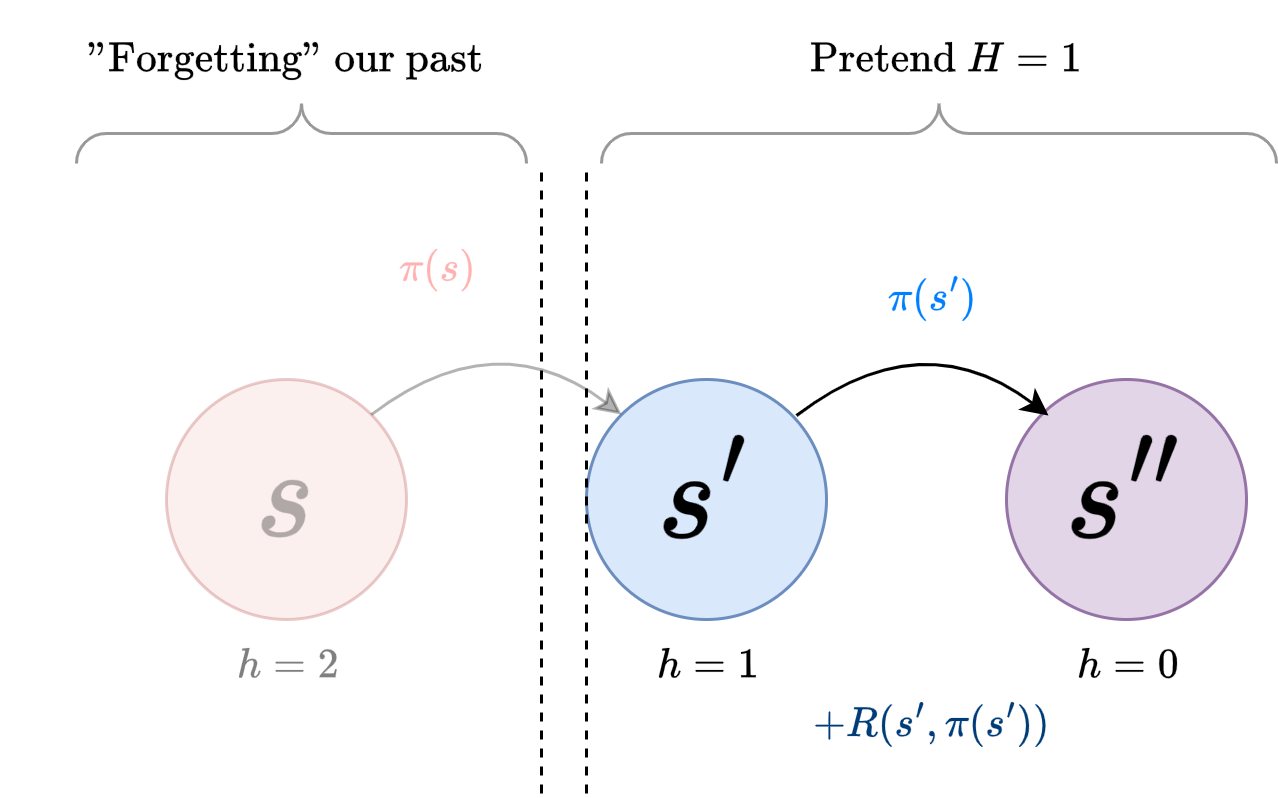
\includegraphics[width=60mm,scale=0.4]{images/mdp_images/h2_forget.png}
            \caption*{Our problem is simpler if we simply "forget" our first step: we just pretend we started at $s'$.}
        \end{figure}

        \begin{itemize}
            \item Now we're in $h=1$. Thankfully, we already computed the optimal policy, $\pi_1^*$.

            \item Our reward will be 
                \note{Since we want the reward, not the action, we'll use "max", not "argmax".}

            \begin{equation}
                R\Big( \blu{s'},\pi_1^*(\blu{s'}) \Big) =
                \max_{\bro{a'}}{ \Big( R\big( \blu{s'},\bro{a'}\big) \Big) }
            \end{equation}

            \item Now, we know the \orgg{second half} of our optimal policy.\\
        \end{itemize}

        \begin{concept}
            The \vocab{optimal} choice of action is independent of previous actions: it's only based on our \redd{state} and \gren{horizon}.

            \begin{itemize}
                \item That means that "\textbf{the last \red{$h$} steps} of a horizon-\blu{$H$} MDP" is \gren{the same} as "\textbf{every step} of a horizon-\red{$h$} MDP"
                \item If we've already computed the optimal policy for a horizon-$h$ MDP, we can \orgg{re-use} them at the end of a \purp{longer horizon}.
            \end{itemize}

            \subsecdiv

            This \purp{simplifies} the search for our \vocab{optimal policy}: we can only focus on policies where those last $n$ steps \gren{match} policy $\pi_n^*$.
        \end{concept}

        \miniex Suppose you know the best way to finish a game of chess in $h$ turns, starting from any position.

        \begin{itemize}
            \item You can use that knowlegde earlier in the game: those will be the end of a longer, winning strategy, starting earlier.
                \note{One weakness of this analogy: in chess, we don't have a well-defined "horizon" for the end of the game. But the same general idea applies.}
        \end{itemize}

        Since we already know the best action, for each state, at $h=1$, we don't have to explore as many possible policies! 

        \subsecdiv

        Now, we can return to our $h=2$ step, with the knowledge of how we'll act in the future. 

        We'll re-introduce our value function, so we can figure out which policy is best:
 
        \begin{equation}
            V_{\grn{\pi}}^{\pur{2}}\big(\red{s} \big) =\quad 
                \overbrace{
                \pur{R} \Big( \red{s},\grn{\pi}\big(\red{s}\big) \Big)
                }^{h=2}
            \;\;+\;\;
                \sum_{\blu{s'}}  
                \;\;
                    \grn{T} \Big( \red{s},\grn{\pi}\big(\red{s}\big),\blu{s'} \Big)
                \;\cdot\; 
                \overbrace{
                \pur{R} \Big( \blu{s'},\grn{\pi}\big(\blu{s'}\big) \Big)
                }^{h=1}
        \end{equation}

        We'll adjust this: 
        
        \begin{itemize}
            \item Our current action is chosen by our policy $\grn{\pi_2}$.
            \item Our next action is chosen by the \orgg{maximum} reward for the $h=1$ step.
        \end{itemize}

        \begin{equation}
            \phantom{V_{\grn{\pi_2}}^{\pur{2}}\big(\red{s} \big) =}\quad 
                \overbrace{
                R \Big( s,\grn{\pi_2}\big(s\big) \Big)
                }^{h=2}
            \;\;+\;\;
                \sum_{s'}  
                \;\;
                    T \Big( s,\grn{\pi_2}\big(s\big),s' \Big)
                \;\cdot\; 
                \overbrace{
                \org{\max_{\bro{a'}}} \Big( R\big( s',\bro{a'}\big) \Big)  \Big)
                }^{h=1}
        \end{equation}



    \phantom{}

    \subsection{Q-Values}

        This is a bit different from $V$, though. Instead of using the \gren{same policy} for every step, we do something different:

        \begin{itemize}
            \item First, we take one \purp{chosen action} $\grn{\pi_2}\big(s\big)$
            \item Then for our \gren{second action}, we choose the optimal policy automatically.
        \end{itemize}

        We'll come up with a new name for this: a \vocab{Q-value function}.\\

        \begin{definition}
            A \vocab{Q-value function} $Q^h\big(\red{s},\bro{a}\big)$ is \textbf{similar} to a value function $V^h_{\pi}\big(\red{s}\big)$, but instead of using the \gren{same policy} for every step, we:

            \begin{itemize}
                \item Choose one action $\bro{a}$
                \item Every choice afterwards is \purp{optimal}.
            \end{itemize}

            This is why the policy $\pi$ has been replaced by a single action $\bro{a}$: you only make \orgg{one choice}, and all following steps are optimal.

            \begin{itemize}
                \item $Q\big(\red{s},\bro{a}\big)$ tells us the \purp{expected reward}, under these conditions.
            \end{itemize}
            
        \end{definition}

        \begin{figure}[H]
            \centering
            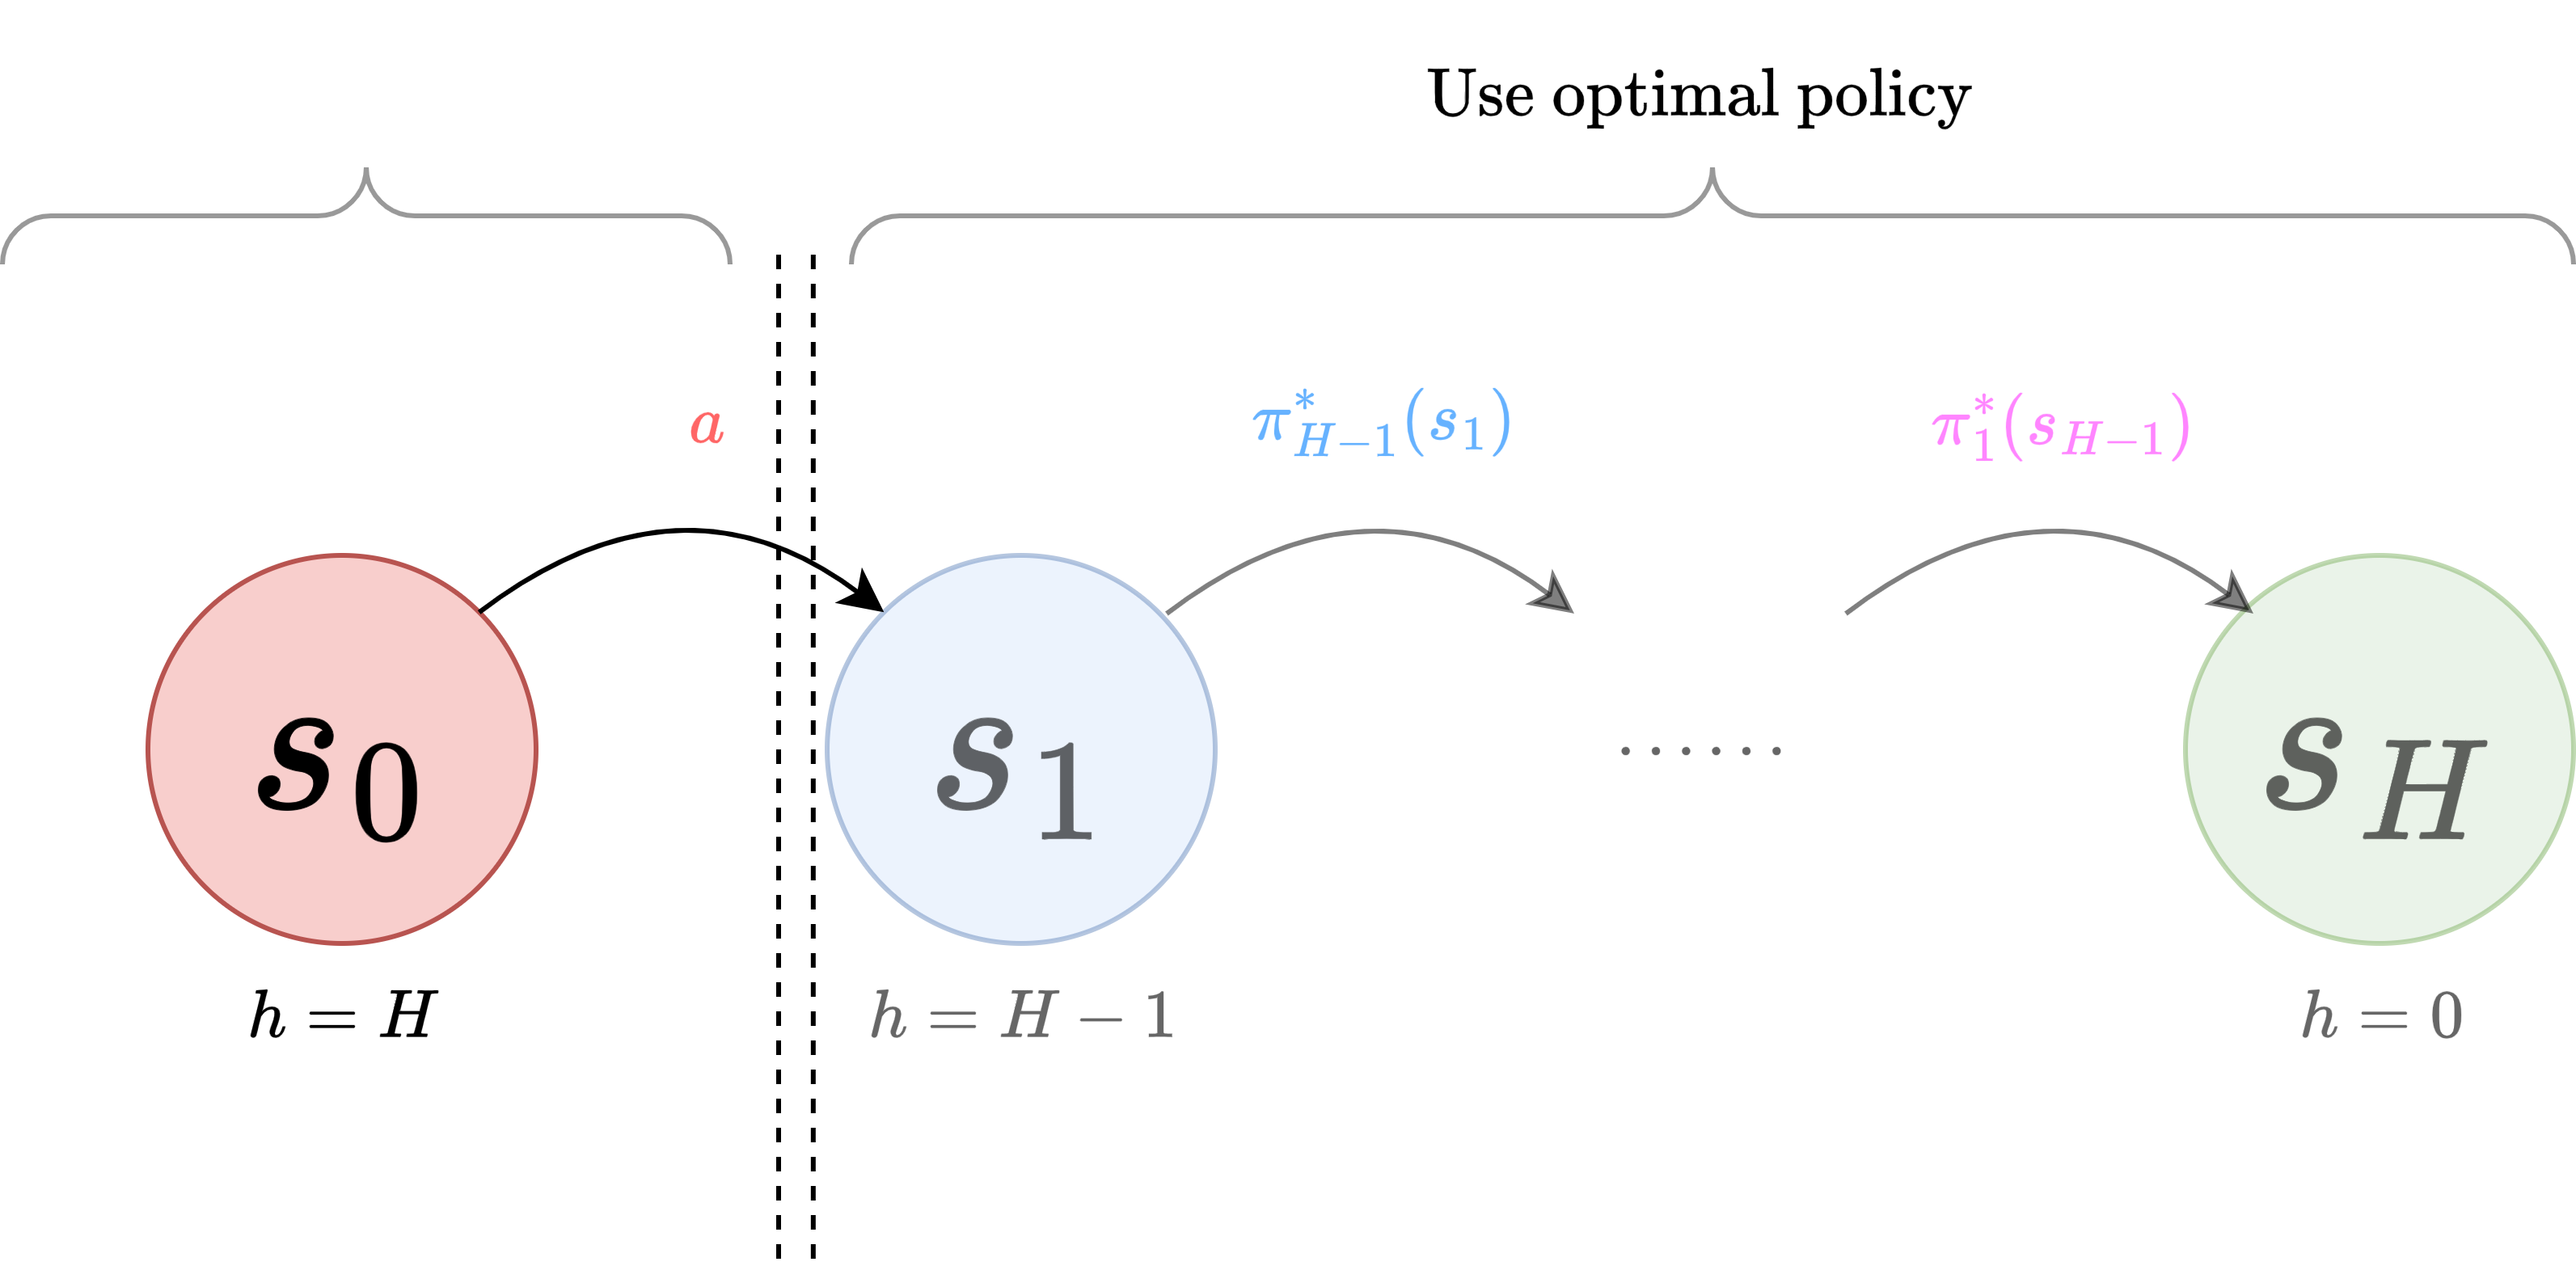
\includegraphics[width=60mm,scale=0.4]{images/mdp_images/q_value.png}
            \caption*{We choose our first action, and the rest are optimal.}
        \end{figure}

        Despite appearing different, the $Q$-value function serves all of the roles we previously needed our value function $V$ for.\\

        \begin{concept}
            We can think of our $Q$-value function $Q^H\big(\red{s},\bro{a}\big)$ as a value function $V^H$ with a \vocab{special kind of policy:}

            \begin{equation*}
                Q^H\big(\red{s},\bro{a}\big) \longrightarrow 
                V^H_\pi\big(\red{s}\big)
            \end{equation*}

            This "special policy" now depends on \purp{horizon}.

            \begin{equation*}
                \pi_h(\red{s}) = 
                \begin{cases}
                    \bro{a} & h=H \\
                    \pi_h^*(\red{s}) & \text{otherwise}
                \end{cases}
            \end{equation*}
        \end{concept}

        This perfectly matches our current strategy: we try out one action $a$, and then rely on the \purp{optimal policies} we developed previously.
            \note{$Q$ can be seen as a way to "try out" one single action, to add onto your, so far, optimal policy.}

        \begin{equation}
            \phantom{V_{\grn{\pi_2}}^{\pur{2}}\big(\red{s} \big) =}\quad 
                \overbrace{
                R \Big( s,\grn{\pi_2}\big(s\big) \Big)
                }^{\text{One action}}
            \;\;+\;\;
                \sum_{s'}  
                \;\;
                    T \Big( s,\grn{\pi_2}\big(s\big),s' \Big)
                \;\cdot\; 
                \overbrace{
                \org{\max_{\pur{a'}}} \Big( R\big( s',\pur{a'}\big) \Big)  \Big)
                }^{\text{Optimal policies}}
        \end{equation}

        If we replace $\grn{\pi_2}\big(s\big)$ with $\bro{a}$, we have our $Q$-value function:

        \begin{equation}
            Q^{\pur{2}}\big(\red{s}, \bro{a} \big) =\quad 
                \overbrace{
                R \Big( s,\bro{a} \Big)
                }^{\text{One action}}
            \;\;+\;\;
                \sum_{s'}  
                \;\;
                    T \Big( s,\bro{a},s' \Big)
                \;\cdot\; 
                \overbrace{
                \org{\max_{\pur{a'}}} \Big( R\big( s',\pur{a'}\big) \Big)  \Big)
                }^{\text{Optimal policies}}
        \end{equation}


    \subsection{$H=2$ completed}

        Our new $Q$-value function already takes care of optimizing $h=1$, so now, we just need to optimize $h=2$: we need to find the \brow{best action} at $h=2$, $a^*$.

        \begin{equation}
            a^* = \bro{\argmax{a}}{} \Big( Q^{\pur{2}}\big(\red{s}, \bro{a} \big) \Big)
        \end{equation}

         \begin{kequation}
            We can use $Q^{\pur{2}}\big(\red{s}, \bro{a} \big)$ to determine the \vocab{optimal policy} for $H=2$.

            \begin{itemize}
                \item $Q^{\pur{2}}\big(\red{s}, \bro{a} \big)$ encodes information about \orgg{immediate} and \purp{future} rewards, while \gren{optimizing} those future steps.
            \end{itemize}
            
            
            This allows us to directly compare different actions $\bro{a}$, searching for an optimal policy:

            \begin{equation*}
                \grn{\pi_2^*}\big(\redd{s}\big) = 
                \bro{a^*} =
                \bro{\argmax{a}}{} \Big( 
                    Q^{\pur{2}}\big(\red{s}, \bro{a} \big) 
                \Big)
            \end{equation*}

            This action will be chosen for our optimal policy $\grn{\pi_2^*}$.
        \end{kequation}

    \subsection{$H=2$ Extended Solution (\redd{Optional})}

        Here's the un-compressed version: it's a lot messier, but it shows more of what's going on.\\

        \begin{remark}
            The \vocab{optimal policy} for horizon $H=2$ comes in two stages:

            \begin{itemize}
                \item We compute the \gren{optimal policy} $\pi_1^*$ and \purp{reward} for our second step, $h=1$.
                    \begin{itemize}
                        \item This tells us how \orgg{valuable} each $h=1$ state $\blu{s'}$ is.
                    \end{itemize}

                \item We compute the \brow{optimal action} $a^*$ for our first step, $h=1$, by factoring in

                    \begin{itemize}
                        \item The \orgg{immediate} reward, $\pur{R} \Big( \red{s},\grn{\pi}\big(\red{s}\big) \Big)$
                        \item The \purp{average rewards in the next step}, based on all possible outcomes.
                    \end{itemize}
            \end{itemize}

                \begin{equation*}
                    \grn{\pi_2^*}\big(\redd{s}\big) = a^* =
                    \bro{\argmax{a}}{} \Bigg\{
                        \overbrace{
                        R \Big( s,\bro{a} \Big)
                        }^{\text{Immediate Reward}}
                        \;\;+\;\;
                        \sum_{s'}  
                        \;\;
                            T \Big( s,\bro{a},s' \Big)
                        \;\cdot\; 
                        \overbrace{
                        \org{\max_{\pur{a'}}} \Big( R\big( s',\pur{a'}\big) \Big)  \Big)
                        }^{\text{(Optimized) Future Reward}}
                    \Bigg\}
                    \end{equation*}

        \end{remark}

        We can see that we \gren{separately} optimize our two steps:
        
        \begin{itemize}
            \item $\pi_1$ first, to get $\pi_1^*$: this gives us our action \bro{$a'$}.

            \begin{equation}
                \org{\max_{\bro{a'}}} \Big( R\big( \blu{s'},\bro{a'}\big) \Big) 
            \end{equation}
            
            \item Then, we use $\pi_1^*$ to find $\pi_2^*$: this gives us our action \pur{$a$}.

            \begin{equation}
                \pur{\argmax{a}{}} \Big( \dots \Big)
            \end{equation}
        \end{itemize}

    \subsection{$H=3$ and beyond}

        Introducing $Q$-values has given us the last tool we need to complete our finite-horizon MDP solution.

        Let's use everything we've built so far:

        \begin{itemize}
            \item After our first step, we're in state $\blu{s'}$, with $H=2$: we already determined what our policy should be, and what the \purp{value} of that policy is:
                \note{The value includes both $h=1$ and $h=2$.}
                
            \begin{equation}
                \grn{\pi_2^*}\big(\blu{s'}\big) = 
                \pur{\argmax{a'}}{} \Big( 
                    Q^{\pur{2}}\big(\blu{s'}, \pur{a'} \big) 
                \Big)
            \end{equation}

            \begin{equation} 
                \text{Optimal Value} = 
                \pur{\max_{a'}} \Big( 
                    Q^{\pur{2}}\big(\blu{s'}, \pur{a'} \big) 
                \Big)
            \end{equation}

            \item Our \purp{first step} is the only one we choose, giving us an immediate reward:

            \begin{equation}
                R \Big( s,\bro{a} \Big)
            \end{equation}
        \end{itemize}

        This matches our description for the $Q$-value function: all we have to do is account for different possible $\blu{s'}$ values, with $ T(s,a,s')$.

        \begin{equation}
            Q^{\pur{3}}\big(\red{s}, \bro{a} \big) 
            \;\;=\;\;
            R \Big( s,\bro{a} \Big)
            \;\;+\;\;
            \sum_{s'}  
                \;\;
                T \Big( s,\bro{a},s' \Big)
                \;\;\cdot\;\;
                \pur{\max_{a'}} \Big( 
                Q^{\pur{2}}\big(\blu{s'}, \pur{a'} \big) 
            \Big)
        \end{equation}

        This strategy, conceptually, works exactly the same, for any possible value of $H$:\\

        \begin{kequation}
            The $Q$-value function for horizon $H$ can be written as:

            

            \begin{equation*}
                Q^{\pur{H}}\big(\red{s}, \bro{a} \big)
                \;\;=\;\; 
                \overbrace{
                    \pur{R} \Big( \red{s},\bro{a} \Big)
                }^{\text{First reward}} 
                \quad+\quad
                \overbrace{
                \sum_{\blu{s'}}  
                        \;\;
                        \underbrace{
                            \grn{T} \Big(   
                            \red{s},\bro{a},\blu{s'} \Big)
                        }_{\text{Chance of } \red{s} \to \blu{s'}}
                        \;\;\; \cdot \;\;\; 
                        \underbrace{
                            \pur{\max_{a'}} \Big( 
                            Q^{\pur{H-1}}\big(\blu{s'}, \pur{a'} \big) \Big)
                        }_{\text{Optimize next step } }
                }^{\text{Future rewards}}
            \end{equation*}

            Or, without extra annotation:

            \begin{equation*}
                Q^{\pur{H}}\big(\red{s}, \bro{a} \big) 
                \;\;=\;\;
                R \Big( s,\bro{a} \Big)
                \;\;+\;\;
                \sum_{s'}  
                    \;\;
                    T \Big( s,\bro{a},s' \Big)
                    \;\;\cdot\;\;
                    \pur{\max_{a'}} \Big( 
                    Q^{\pur{H-1}}\big(\blu{s'}, \pur{a'} \big) 
                \Big)
            \end{equation*}

            Note that horizon $H$ relies on optimizing horizon $H-1$, similar to value iteration.
        \end{kequation}

        And based on this $Q$-value, we can determine the optimal action for our current state (and thus, our \purp{optimal policy}):\\

        \begin{kequation}
            We can use $Q^{\pur{H}}\big(\red{s}, \bro{a} \big)$ to determine the \vocab{optimal policy} for horizon $H$.

            \begin{equation*}
                \grn{\pi_H^*}\big(\redd{s}\big) = 
                \bro{\argmax{a}}{} \Big( 
                    Q^{\pur{H}}\big(\red{s}, \bro{a} \big) 
                \Big)
            \end{equation*}

            We can use this form of equation to get \orgg{every optimal policy}.
        \end{kequation}

        Note some important reminders. First, make sure to distinguish between $Q$ and $V$.\\

        \begin{clarification}
            Let's compare our \purp{value function} equation $V$, to our \gren{$Q$-value function} equation:

            \begin{itemize}
                \item For our $Q$-value, we choose \bro{one action}, and the remainder are \purp{optimal}.
            \end{itemize}

            \begin{equation*}
                Q^{\pur{H}}\big(\red{s}, \bro{a} \big) 
                \;\;=\;\;
                R \Big( s,\bro{a} \Big)
                \;\;+\;\;
                \sum_{s'}  
                    \;\;
                    T \Big( s,\bro{a},s' \Big)
                    \;\;\cdot\;\;
                    \pur{\max_{a'}} \Big( 
                    Q^{\pur{H-1}}\big(\blu{s'}, \pur{a'} \big) 
                \Big)
            \end{equation*}
            
            \begin{itemize}
                \item Meanwhile, $V$ relies on the \gren{same policy $\pi$} for all actions.
            \end{itemize}

        
            \begin{equation*}
                V_{\grn{\pi}}^{\pur{H}}\big(\red{s} \big) \;\;=\;\; 
                    \pur{R} \Big( \red{s},\grn{\pi}\big(\red{s}\big) \Big)
                \quad+\quad
                \sum_{\blu{s'}}  
                        \;\;
                            \grn{T} \Big(   
                            \red{s},\grn{\pi}\big(\red{s}\big),\blu{s'} \Big)
                        \;\;\; \cdot \;\;\; 
                            V_{\grn{\pi}}^{\pur{H-1}}\big(\blu{s'} \big)
            \end{equation*}

            
        \end{clarification}

        \begin{figure}[H]
            \centering
            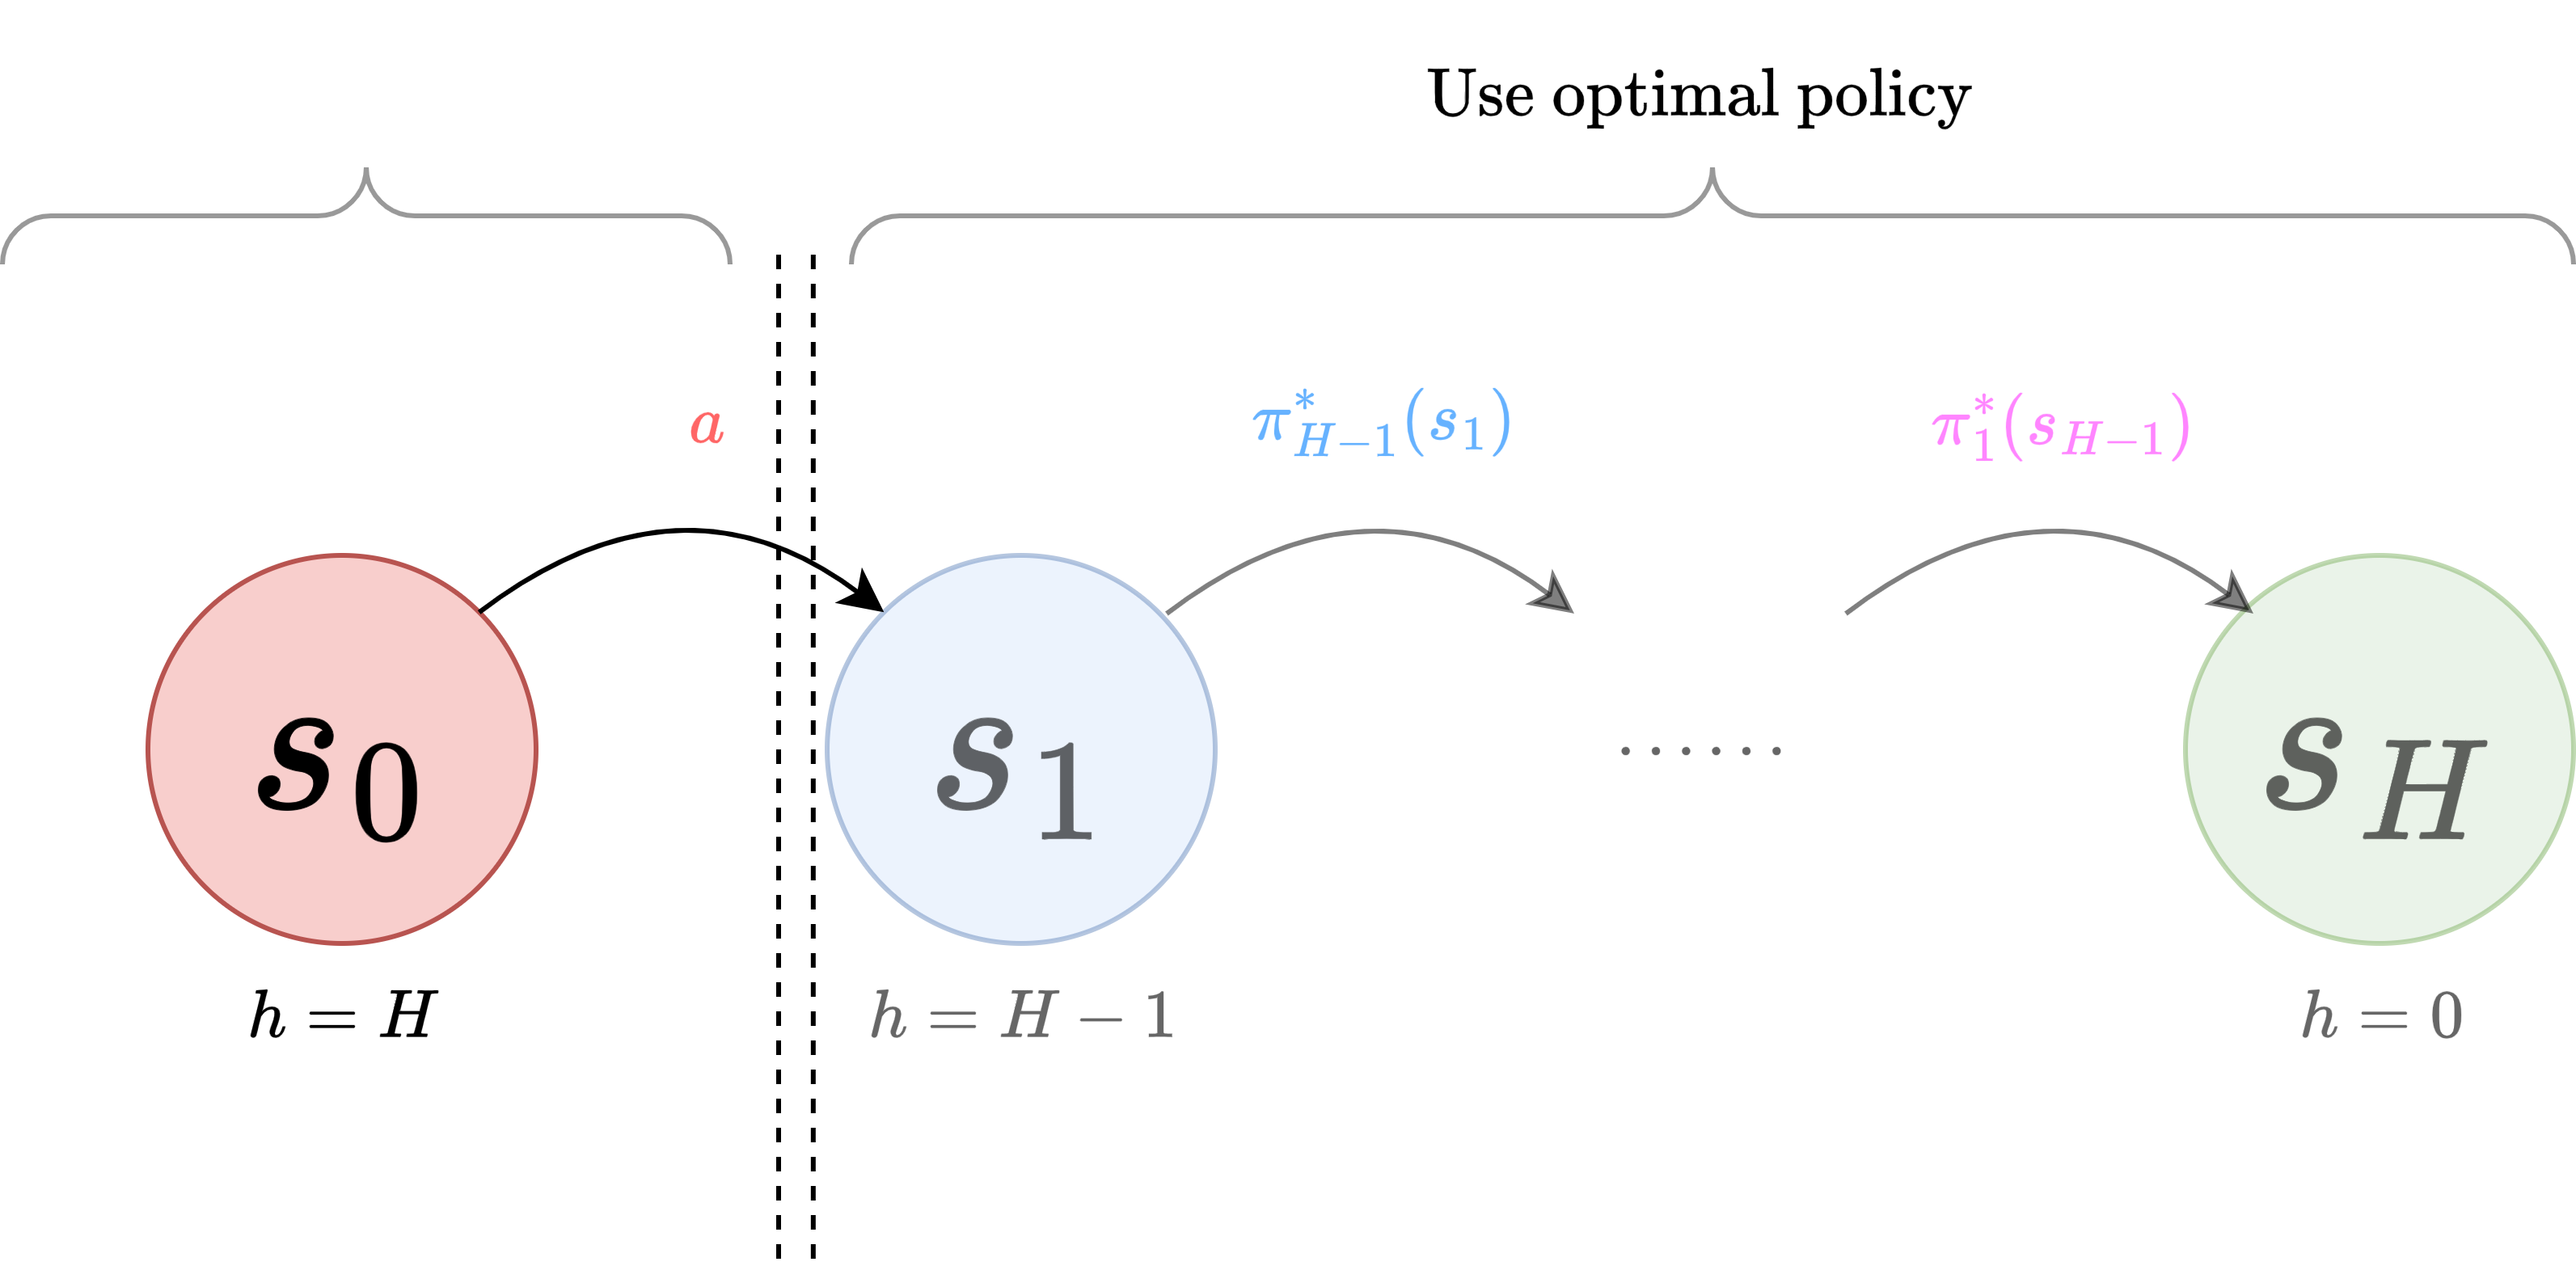
\includegraphics[width=70mm,scale=0.4]{images/mdp_images/q_value.png}
            \caption*{Our first action is chosen manually: after that, we use an optimal policy.}
        \end{figure}

        \begin{figure}[H]
            \centering
            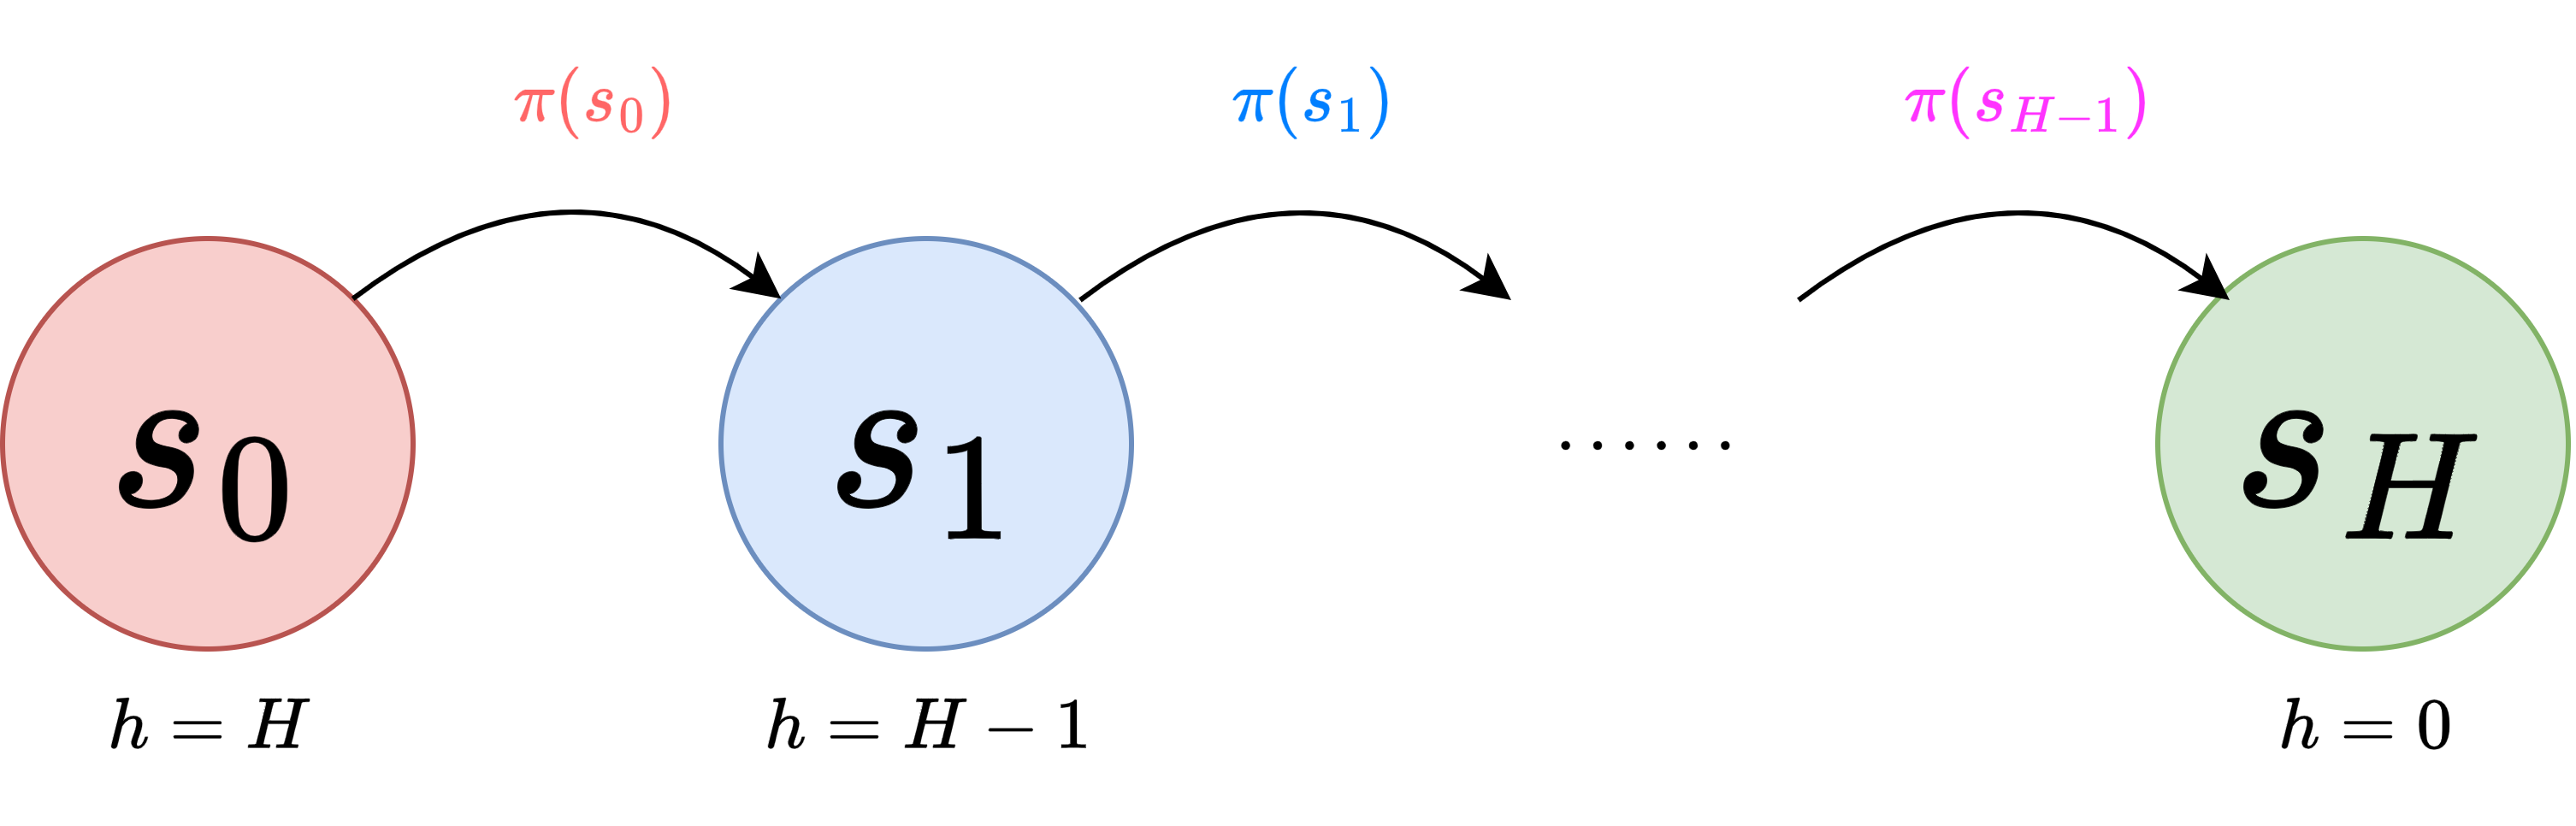
\includegraphics[width=60mm,scale=0.4]{images/mdp_images/v_value.png}
            \caption*{All of our actions are chosen by our (potentially non-optimal) policy $\pi$.}
        \end{figure}

    \pagebreak

    \subsection{Finite-Horizon $Q$-Value MDP solution}

        We have a method for creating the optimal policy:

        \begin{itemize}
            \item Choose any action for $\pi_0^*(s)$.
            \item Maximize $R(s,a)$ for $a=\pi_1^*(s)$
            \item Maximize $Q(s,a)$ for $a=\pi_h^*(s)$, if $h\geq 2$.
        \end{itemize}

        For horizon $H$, we can \orgg{re-use} the optimal policies for shorter horizons.

            \begin{itemize}
                \item This concept is encoded by the way $Q$-values work.

                \item So, we can use these $Q$-values to find the optimal policy:
            \end{itemize}

        

        So, our focus is on those $Q$-values. We'll compute them as we progressively increase the horizon:

        \begin{equation}
            \org{Q^{0}\big(s,a \big)}  \;\;=\;\; 
            0
        \end{equation}

        \begin{equation}
            \pur{Q^{1}\big(s,a \big)} \;\;=\;\; 
                    R \Big( s,\pi\big(s\big) \Big)
                + \org{0}
        \end{equation}

        \begin{equation}
            \red{Q^{2}\big(s,a \big)} \;\;=\;\; 
                    R \Big( s,a \Big)
                \;\;+\;\
                    \pur{\sum_{s'}}  
                        \;\;
                        T \Big(          s,\pi\big(s\big),s' \Big)
                        \;\cdot\; 
                        \bro{ \max_{a'} \Big( \pur{Q^{1}\big(s',a' \big)} \Big)}
        \end{equation}

        And if we keep going...

        \begin{equation}
            \grn{Q^{H}\big(s,a \big)} \;\;=\;\; 
                    R \Big( s,a \Big)
                \;\;+\;\;
                    \red{\sum_{s'}}  
                        \;\;
                        T \Big(          s,\pi\big(s\big),s' \Big)
                        \;\cdot\; 
                        \bro{ \max_{a'} \Big( \red{Q^{H-1}\big(s',a' \big)} \Big)}
        \end{equation}

    \subsection{Dynamic Programming}

        For value function $V$ and $Q$-values, we've been using a very particular strategy for computing our solutions.

        \begin{itemize}
            \item We solve \purp{simpler subproblems} (like $V^1$) and \gren{save the results}.
            \item Later, we \orgg{re-use} those solutions for more complicated problems (like $V^2$).
        \end{itemize}

        This saves us a lot of work: 
        
        \begin{itemize}
            \item \miniex We could re-compute all the $V^1$ values, every time we need a $V^2$ value.
            \item But if, instead, we just store those values and use them later, we save them.
            \item The benefits are more obvious for computing $V^{200}$: it would be a nightmare to have to consider every possible sub-problem.
                \note{We don't have to pay attention to $V^{2}$ when doing $V^{200}$: that information is stored in $V^{199}$.}
        \end{itemize}

        We call this strategy \vocab{dynamic programming}, despite it being neither "dynamic", nor "programming".\\

        \begin{definition}
            \vocab{Dynamic Programming} is a strategy for solving complex problems that can be broken up into simpler, similar problems ("subproblems").

            \begin{itemize}
                \item First, we solve the \purp{subproblems}, and \gren{save} the result. 

                \item These "mini-solutions" are re-used as a part of larger, more \textbf{complicated} problems.
            \end{itemize}

            Because a single sub-solution can be used \orgg{many times}, you save time by storing the answer, rather than re-computing it every time you need it.
            
        \end{definition}

        We use it for every step of our value/$Q$-value calculation: 

        \begin{equation}
            \grn{Q^{H}\big(s,a \big)} \;\;=\;\; 
                    R \Big( s,a \Big)
                \;\;+\;\;
                    \red{\sum_{s'}}  
                        \;\;
                        T \Big(          s,\pi\big(s\big),s' \Big)
                        \;\cdot\; 
                        \bro{ \max_{a'} \Big( \red{Q^{H-1}\big(s',a' \big)} \Big)}
        \end{equation}

        $Q^H$ always requires us to use $Q^{H-1}$.

        \begin{itemize}
            \item $Q^H(s,a)$ has an equation for each state-action pair $(s,a)$. 
            
            \begin{itemize}
                \item Each of these equations will use $Q^{H-1}$: that involves using $Q^{H-1}$ \purp{many times}.
            \end{itemize}
            
            \item It would be much slower if, for every $Q^H(s,a)$, we had to \gren{re-compute} all of $Q^{H-1}$.
        \end{itemize}



    \pagebreak

    \subsection{Dynamic Programming Performance (\redd{Optional})}

        Let's compare the performance of working with, and without dynamic programming. Our goal is to compute $Q^h(s,a)$.

        \begin{equation}
            |\mathcal{S}|=m, \qquad |\mathcal{A}|=n
        \end{equation}

        We'll need this concept:\\

        \begin{concept}
            If we have a pair of elements, $(a,b)$, the total number of \purp{possibilities} is:

            \begin{itemize}
                \item The number of possible $a$ values, \gren{times} the number of possible $b$ values.
            \end{itemize}

            This idea works for larger sequences: you just multiply together the \purp{possible choices} at each step.
        \end{concept}

        We'll count the amount of work we need with, and without dynamic programming.


        \subsecdiv

        First: \orgg{without dynamic programming}.

        One way to compute the value of $Q^H(s,a)$ is to consider \purp{every possible outcome} of that action, and find the optimal one.

        \begin{itemize}
            \item \gren{How many} outcomes are there? One outcome has one \textbf{state-action pair} ($mn$ pairs), for each \textbf{timestep} ($h$ timesteps).
                \note{$m$ states, $n$ actions: $mn$ pairs of states and actions.}
        \end{itemize}

        The total number of possible outcomes is $(mn)^h$. So, our total work is proportional to that:
            \note{At each step, we have $mn$ possible pairs. So, for two timesteps, we have to choose from $mn$ options, twice: $(mn)^2$.}

        \begin{equation}
            O\big((mn)^h\big)
        \end{equation}

        We won't teach $O$-notation here.

        \subsecdiv

        Let's \orgg{use dynamic programming} this time.

        \begin{itemize}
            \item For our \purp{final timestep}, we have $mn$ possible state-action pairs. We pick the optimal action for each state, and we \gren{save} its value as $Q^h(s,a)$.
            \item For our previous timestep, we \purp{don't care} about the possibilities in the final timestep: we just trust $Q^h(s,a)$, and use it to select one of our $mn$ actions. 
        \end{itemize}

        So, at each timestep, we compare $mn$ elements: we don't have to consider combinations across different timesteps.

        However, we do still have to do this calculation once per timestep: $h$ times. We get $mnh$.

        \begin{equation}
            O\big(mnh\big)
        \end{equation}

        \begin{concept}
            Using \vocab{dynamic programming} for $Q$-value computation dramatically increases \gren{efficiency}.

            Instead of taking $O\big((mn)^h\big)$ time, we need $O\big(mnh\big)$ time.

            \begin{itemize}
                \item That's \orgg{exponentially} faster!
            \end{itemize}
        \end{concept}

        In short: the difference is that dynamic programming allows us to "ignore" other timesteps, and just rely on $Q$-values.

        \begin{itemize}
            \item Without dynamic programming, we have to "remember" other timesteps, and consider \purp{combinations} of state-action pairs.
        \end{itemize}





    \pagebreak

    \subsection{Optimal Policies -- Infinite Horizon}

        Now, we need to figure out how to get the optimal \purp{infinite-horizon} policy.

        We'll start off with our finite $Q$-value equation:

        \begin{equation}
            \grn{Q^{H}\big(s,a \big)} \;\;=\;\; 
                    R \Big( s,a \Big)
                \;\;+\;\;
                    \red{\sum_{s'}}  
                        \;\;
                        T \Big(          s,\pi\big(s\big),s' \Big)
                        \;\cdot\; 
                        \bro{ \max_{a'} \Big( \red{Q^{H-1}\big(s',a' \big)} \Big)}
        \end{equation}

        All we do is \purp{remove the horizon}, and \gren{add the discount factor}. 
    
        \begin{equation}
            \grn{Q\big(s,a \big)} \;\;=\;\; 
                    R \Big( s,a \Big)
                \;\;+\;\;
                \gamma
                \grn{\sum_{s'}}  
                    \;\;
                    T \Big(          s,\pi\big(s\big),s' \Big)
                    \;\cdot\; 
                    \bro{ \max_{a'} \Big( \grn{Q\big(s',a' \big)} \Big)}
        \end{equation}

        Now, our $Q$-value function is an equation of \purp{itself}.\\

        \begin{kequation}
            The \vocab{$Q$-value function} for \purp{infinite horizon} can be written as:

            \begin{equation*}
                \grn{Q\big(s,a \big)} \;\;=\;\; 
                        R \Big( s,a \Big)
                    \;\;+\;\;
                    \gamma
                    \grn{\sum_{s'}}  
                        \;\;
                        T \Big(          s,\pi\big(s\big),s' \Big)
                        \;\cdot\; 
                        \bro{ \max_{a'} \Big( \grn{Q\big(s',a' \big)} \Big)}
            \end{equation*}
        \end{kequation}

        Something similar happened before, when we were doing value functions. Why is that?

        \begin{itemize}
            \item We're in the \redd{same situation} before and after we take one (successful) step: we \purp{don't know} how long it will be until the model terminates.
            \item In fact, nothing has changed: the chance of failing after one more step is still $\gamma$.
        \end{itemize}

        Because "maximizing $Q$" is how we determine our policy, we see that:\\

        \begin{concept}
            The optimal policy for an \purp{infinite-horizon MDP} is \gren{the same}, at any timestep, regardless of past events.

            We call this a \vocab{stationary} optimal policy, because it doesn't change over time.
        \end{concept}

        Our goal is to look for one of these "stationary" optimal policies.
            \note{There can be several optimal policies. We're only looking for one.}

    \subsection{Finding an Optimal Policy}

        We have a problem, though. When computing the \purp{infinite value function}, we were able to solve a system of \gren{linear equations}.

        But our $Q$-value function is \gren{non-linear} this time, because of the \brow{max} operation. We can't solve that!

    

        

    

        


        

        

        

        

    




\pagebreak

\section{Old Material}



%%%%%%%%%%%%%%%%%%%%%%%%%%%%%%%%%%%%%%%%%%%%%%%%%%%%%%%%%%%%%%%%%%%%%%%%%%%%%
\section{Finding policies for MDPs}


%%%%%%%%%%%%%%%%%%%%%%%%%%%%%%%%%%%%%%%%
\subsection{Finding optimal infinite-horizon policies}
\label{sec:mdp_infinite_horizon_optimal}

In contrast to the finite-horizon case, the best way of behaving in an
infinite-horizon discounted {\sc mdp} is not time-dependent: at every
step, your expected future lifetime, given that you have survived
until now, is $1 / (1 - \gamma)$.
%
\question{
Verify this fact:  if, on every day you wake up, there is a
probability of $1 - \gamma$ that today will be your last day, then your
expected lifetime is $1 /  (1 - \gamma)$ days.
}

An important theorem about {\sc mdp}s is: in the infinite-horizon case, there exists a stationary\index{policy!stationary policy}
\note{Stationary means that it doesn't change over time; in contrast, the
  optimal policy in a finite-horizon {\sc mdp} is {\em non-stationary.}}
optimal policy $\pi^*$ (there may be more than one) such that for all
$s \in \mathcal S$ and all other policies $\pi$, we have 
\begin{equation}
 V_{\pi^*}(s) \ge V_{\pi}(s) \;\;.
\end{equation}

% Let $n = |\mathcal S|$ andd $m = |\mathcal A|$. Algorithm for finding $\pi^*$:
% \begin{itemize}
% \item
% enumerate and test, complexity is $O(m^n)$
% \item
% linear programming, complexity is $O(\text{poly}(n, m b))$ where $b$ is the number of bits per element of $T, R$
% \item
% policy iteration, complexity is $O(\text{poly}(n, m, \text{bits}(\gamma)))$, requires solving lots of $n \times n$ systems
% \item
% {\underline{value iteration}}, complexity is $O\left(\text{poly}(n, m, b, \frac{1}{1 - \gamma}\right)$
% \end{itemize}
% The latter is easy to implement and the foundation for many reinforcement-learning methods.

There are many methods for finding an optimal policy for an {\sc mdp}.
We have already seen the finite-horizon value iteration case.  Here we
will study a very popular and useful method for the infinite-horizon
case, {\em infinite-horizon value iteration}.  It is also important to
us, because it is the basis of many {\em reinforcement-learning}
methods.

Define $Q^*(s, a)$ to be the expected infinite-horizon discounted
value of being in state $s$, executing action $a$, and executing
an optimal  policy $\pi^*$ thereafter.  Using similar reasoning to the
recursive definition  of  $V_\pi$,  we can express this value
recursively as
\begin{equation}
 Q^*(s, a) = R(s, a) + \gamma\sum_{s'}T(s, a, s')\max_{a'}Q^*(s',
a') \;\;.
\end{equation} 
This is also a set of equations, one for each $(s, a)$ pair.  This
time, though, they are not linear, and so they are not easy to solve.
But there is a theorem  that says they have a unique solution!

If we knew the optimal action-value function, then  we could derive an
optimal policy  $\pi^*$ as
\begin{equation}
 \pi^*(s) = \text{arg}\max_{a}Q^*(s, a) \;\;.
\end{equation}
\question{The optimal value function is unique, but the optimal policy
  is not.  Think of a situation in which there is more than one
  optimal policy.}

We can iteratively solve for the $Q^*$ values with the infinite-horizon
value iteration algorithm, shown below:

\begin{codebox}
  \Procname{$\proc{Infinite-Horizon-Value-Iteration}(\mathcal S, \mathcal A, T, R, \gamma, \epsilon)$}
  \li     \For $s \in \mathcal{S}, a \in \mathcal{A}:$
	\Do
  \li        $Q_{\text{old}}(s, a) = 0$
        \End
  \li     \While True:
        \Do
  \li        \For $s \in \mathcal{S}, a \in \mathcal{A}:$
           \Do
  \li           $Q_{\text{new}}(s, a) = R(s, a) + \gamma\sum_{s'}T(s, a, s')\max_{a'}Q_{\text{old}}(s', a')$
         \End

  \li      \If $\max_{s, a}\lvert Q_{\text{old}}(s, a) - Q_{\text{new}}(s, a)\rvert < \epsilon:$
         \Do
  \li           return $Q_{\text{new}}$
        \End
  \li      $Q_{\text{old}} = Q_{\text{new}}$
	\End
\end{codebox}

\paragraph*{Theory}

There are a lot of nice theoretical results about infinite-horizon value iteration.
For some given (not necessarily optimal) $Q$ function, define
$\pi_{Q}(s) = \text{arg}\max_{a}Q(s, a)$.   
\begin{itemize}
\item After executing infinite-horizon value
iteration with parameter $\epsilon$,  
\note{Note the new 
  notation!  Given two functions $f$ and $f'$, we
  write $\lVert f - f' \rVert_\text{max}$ to mean $\max_x \lvert f(x)
  - f'(x)\rvert$.   It measures the maximum absolute
  disagreement between the two functions at any input $x$.}
\begin{equation}
\lVert  V_{\pi_{Q_{\text{new}}}} - V_{\pi^*} \rVert_{\text{max}} < \epsilon \;\; .
\end{equation}
%
\item
There is a value of $\epsilon$ such that
\begin{equation}
 \Vert Q_{\text{old}} - Q_{\text{new}} \rVert_{\text{max}} <
\epsilon \Longrightarrow \pi_{Q_{\text{new}}} = \pi^* 
\end{equation}  
\item  As the algorithm executes,   
$\lVert V_{\pi_{Q_{\text{new}}}} - V_{\pi^*} \Vert_{\text{max}}$ decreases
monotonically on each iteration.
\item The algorithm  can be executed asynchronously, in parallel: as
  long as all $(s, a)$ pairs are updated infinitely often in an
  infinite run, it still converges to optimal value. 
\note{This is very important for reinforcement learning.}

\end{itemize}

%%% Local Variables:
%%% mode: latex
%%% TeX-master: "top"
%%% End:
